\section{Количество бутстреп репликаций $B$}

Насколько большим мы должны взять $B$, количество бутстреп репликаций, используемых для оценки $\widehat{se}_B$? Идеальная бутстреп оценка $\widehat{se}_\infty$ использует $B=\infty$, и в этом случае $\widehat{se}_\infty$ равно плагин оценке $se_{\hat F}(\hat\theta^*)$. Формула (5.12) дает $\widehat{se}_\infty$ для $\hat\theta=\bar x$, но для большинства других статистических данных мы должны фактически выполнить генерацию бутстреп выборок. Время, затрачиваемое компьютером, которое в основном зависит от того, сколько времени требуется для оценки бутстреп репликаций (6.5), линейно увеличивается с $B$. Временные ограничения могут диктовать небольшое значение $B$, если $\hat\theta = s (\mathbf{x})$ -- очень сложная функция.

Нам нужно такое же хорошее поведение от оценки стандартной ошибки, что и от оценки любой другой интересующей величины: небольшая систематическая ошибка и небольшое стандартное отклонение. Бутстреп оценка стандартной ошибки обычно имеет относительно небольшое смещение. Идеальная начальная оценка $\widehat{se}_\infty$ имеет наименьшее возможное стандартное отклонение среди почти несмещенных оценок $se_F(\hat\theta)$, по крайней мере, в асимптотическом $(n \rightarrow\infty)$ смысле. Эти хорошие свойства вытекают из того факта, что $\widehat{se}_\infty$ -- это плагин оценка $se_{\hat F}(\hat\theta)^*$. Нетрудно показать, что $\widehat{se}_B$ всегда имеет большее стандартное отклонение, чем $\widehat{se}_\infty$. Практический вопрос: насколько большее?

Приблизительный, но вполне удовлетворительный ответ можно сформулировать в терминах коэффициента вариации $\widehat{se}_B$, отношения стандартного отклонения $\widehat{se}_B$ к его математическому ожиданию. Повышенная изменчивость из-за остановки после $B$ бутстреп репликаций, а не бесконечности, отражается в увеличенном коэффициенте вариации,
\begin{equation}
    cv(\widehat{se}_B)=\left\{cv(\widehat{se}_\infty)^2+\frac{E(\Delta)+2}{4B}\right\}^{1/2}.
\end{equation}
Здесь $\Delta$ -- параметр, который измеряет, насколько длиннохвостым является распределение $\hat\theta^*$: если $\Delta$ равно нулю для нормального распределения, оно колеблется от $-2$ для короткохвостых распределений до произвольно больших значений, когда F длиннохвостное. На практике $\delta$ обычно не превышает $10$. Коэффициент вариации в уравнении (6.9) относится к вариации как на уровне повторных выборок (бутстреп), так и на уровне исходной выборки. Идеальная оценка $\widehat{se}_\infty = se_{\hat F}(\hat\theta^*)$ не идеальна. Она все еще может иметь значительную изменчивость в качестве оценки $se_F(\hat\theta)$ из-за изменчивости $\hat F$ как оценки $F$. Например, если $x_1, x_2, \cdots, x_n$ является случайной выборкой из нормального распределения и $\hat\theta=\bar x$, тогда $cv(\widehat{se}_\infty)=1/\sqrt{2n}$, равное $0.22$ для n = 10. Формула (6.9) имеет важное практическое следствие: для значений $cv(\widehat{se}_\infty)$ и $\Delta$, которые могут возникнуть на практике, $cv(\widehat{se}_B)$ не намного больше, чем $cv(\widehat{se}_\infty)$ для $B\ge 200$. 

Таблица 6.2 сравнивает $cv(\widehat{se}_B)$ с $cv(\widehat{se}_\infty)$ для различных вариантов $B$, предполагая $\Delta = 0$. Очень часто можно ожидать, что $cv(\widehat{se}_\infty)$ будет не меньше, чем $0.10$, и в этом случае $B = 100$ дает вполне удовлетворительные результаты.
\newline

\noindent
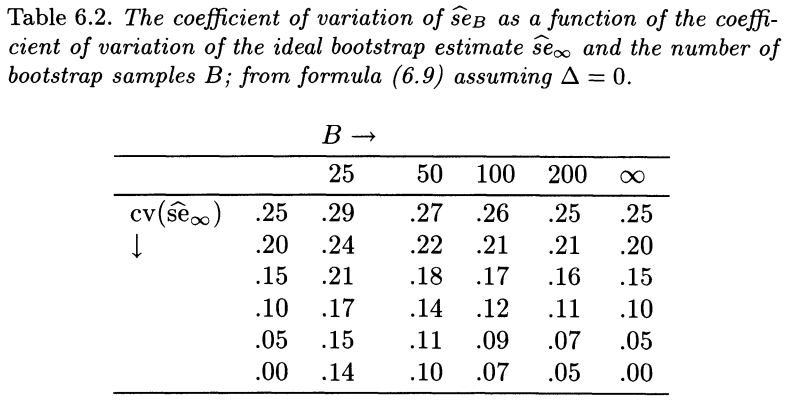
\includegraphics[width=\linewidth]{5/t62.png}
\newline
Вот два практических правила, взятых из опыта:
\begin{enumerate}
    \item Даже небольшое количество бутстреп репликаций, скажем, $B = 25$, обычно является информативным. $B = 50$ часто бывает достаточно, чтобы дать хорошую оценку $se_F (\hat\theta)$.
    \item Очень редко для оценки стандартной ошибки требуется более $B = 200$ репликаций. (Для доверительных бутстреп интервалов требуются гораздо большие значения $B$.) 
\end{enumerate}

Аппроксимации, полученные путем случайной выборки или моделирования, называются оценками Монте-Карло. Вычислительные методы, отличные от прямого моделирования Монте-Карло, иногда могут во много раз сократить количество повторений $B$, необходимых для достижения заданной точности. Между тем стоит помнить, что бутстреп данные, как и реальные данные, заслуживают внимательного изучения. В частности, отображение гистограммы бутстреп репликаций почти никогда не бывает пустой тратой времени. 